%% Overleaf			
%% Software Manual and Technical Document Template	
%% 									
%% This provides an example of a software manual created in Overleaf.

\documentclass{ol-softwaremanual}

% Packages used in this example
\usepackage{graphicx}  % for including images
\usepackage{microtype} % for typographical enhancements
\usepackage{minted}    % for code listings
\usepackage{amsmath}   % for equations and mathematics
\setminted{style=friendly,fontsize=\small}
\renewcommand{\listoflistingscaption}{List of Code Listings}
\usepackage{hyperref}  % for hyperlinks
\usepackage[a4paper,top=4.2cm,bottom=4.2cm,left=3.5cm,right=3.5cm]{geometry} % for setting page size and margins

% Custom macros used in this example document
\newcommand{\doclink}[2]{\href{#1}{#2}\footnote{\url{#1}}}
\newcommand{\cs}[1]{\texttt{\textbackslash #1}}

% Frontmatter data; appears on title page

%\title{\vspace{30} Automated Machine Learning Multiple Imputation with \\\texttt{MLIM}}
\title{\vspace{30} \texttt{MLIM} Multiple Imputation Handbook}
\version{\texttt{0.0.8}}

\author{E. F. Haghish\\ \small{Department of Psychology\\University of Oslo, Norway \\ haghish@uio.no}\linebreak}

\softwarelogo{
\includegraphics[width=8cm]{figures/mlim.png}}

\begin{document}

\maketitle

\tableofcontents
\listoflistings
\newpage

\section{Introduction}

\texttt{mlim} is a multiple imputation software package for \textbf{R} language, which uses automated machine learning to fine-tune the models and minimize the imputation error. In addition, \texttt{mlim} uses state-of-the-art computer science procedures to auto-balance imbalance data (see below), which results to fairer imputation, when one category is less represented or appears with lower prevalence. The latter can increase the coefficients estimated from imputed data, which is a big advantage for moving toward automated machine learning solutions for multiple imputations. The difference between \texttt{mlim} \texttt{mlim} automatically fine-tunes the model for imputing each variable, hence, the user is not required to define the parameters of the model and instead, the model is optimized for each variable, while avoiding overfitting. These features, to the author's knowledge, had not been implemented in any R package before. 

This document provides a nice and clean documentation of the package and is occasionally updated with new stable releases. Visit the \doclink{https://github.com/haghish/mlim}{\texttt{mlim} repository on GitHub} to access more materials and tutorials about the package.



\subsection{Automated machine learning for missing data imputation}

In recent years, there have been several attempts for using machine learning for missing data imputation. Yet, \texttt{mlim} is unique because it is the first \textbf{R} package to implement automated machine learning for multiple imputation and brings the state-of-the-arts of machine learning to provide a versatile missing data solution. But how is automated machine learning any different from other machine learning imputation models? The difference is that automated machine learning algorithms \textit{fine-tune} the models, resulting in more accurate predictions, in contrast to classical (static) machine learning models, where the model's parameters should be specified by the user. When it comes to missing data imputation, instead of setting up an algorithm with pre-specified parameters to impute all the variables of the dataset with the same parameters, we can allow the algorithm to effectively search for the optimal parameters for each variable. This dramatic change in approaching missing data imputation should explain why \texttt{mlim} outperforms other \textbf{R} packages because it optimizes the imputation of each variable. Compared to other \textbf{R} packages, \texttt{mlim} provides a better multiple imputation procedure because: 

\begin{enumerate}
    \item It automatically fine-tunes the parameters of each machine learning model for each variable
    
    \item It delivers a higher prediction accuracy, hence, lower imputation error
    
    \item It is a fairer algorithm to minorities, correcting for biases emerging from imbalanced data
    
    \item Does not make any assumption about the distributions of the variables
    
    \item Takes the interactions between the variables into account
    
    \item Does not enforce linear relations between the predictors
    
    \item Uses a blend of different machine learning models
    
    \item Implements a sophisticated procedure for optimizing imputed data with different algorithms

\end{enumerate}






\subsection{Installation}

\texttt{mlim} is under fast development. The package receive monthly updates on CRAN. Therefore, it is recommended that you install the GitHub version until version 0.1 is released. To install the latest development version from GitHub:

%\begin{listing}
%\inputminted{octave}{code/BitXorMatrix.m}
%\caption{Example from external file}
%\label{listing:octave}
%\end{listing}

\begin{listing}[h]
\begin{minted}{R}
# install mlim from GitHub
library(devtools)
install_github("haghish/mlim")

# install mlim from CRAN
install.packages("mlim")
\end{minted}
%\caption{installing mlim R package}
\label{listing:r}
\end{listing}


\section{Procedure}

\texttt{mlim} support several algorithms. These algorithms have different computational needs and \texttt{mlim} optimizes the imputation procedure without requiring excessive computational resources. These algorithms, their computational requirements, and \texttt{mlim} optimization procedure is further explained below.

\subsection{Imputation steps}

\texttt{mlim} follows three steps to carry out the imputation:

\begin{enumerate}
    \item \textbf{Preimputation} : Instead of replacing missing observations with mean or mdoe, a very fast \textbf{RF} (Random Forest) algorithm is used to carry out a primary single imputation. The imputed data will be further optimized in the following steps.
    \item \textbf{Reimputation} : The preimputed data will be reimputed with \textbf{ELNET} (default) or another algorithm. 
    \item\textbf{Postimputation} : The reimputed data can be even further optimized using a heavier algorithm that requires much more computational resources such as \textbf{GBM}, \textbf{XGB}, \textbf{DL}, or all of them via \textbf{Ensemble}. The latter trains a stacked ensemble from all of the available trained algorithms to minimize imputation error as much as possible, within the given fine-tuning time. \textbf{\color{violet}Note: Using 'Ensemble' is not recommended for general imputation practice and is intended for particular cases or smaller datasets were minimizing imputation error can make a significant difference.}
\end{enumerate}

\subsection{Preimputation, reimputation, and postimputation}

although the third step is optional. The algorithm begins with a preimputation, which is a quick imputation with Random Forest. The reason for pre-imputation is to save time on the reimputation. Therefore, instead of replacing missing observations with mean and mode and starting a slow procedure for optimizing the imputed values, a fast and efficient algorithm is used for initial imputation and then, the imputed values are optimized. For the second step, the \texttt{ELNET} algorithm is fine-tuned. Note that what makes \texttt{ELNET} slower than Random Forest is the fact that \texttt{ELNET} is being fine-tuned but the preimputation procedure is not fine-tuned and a fixed model is used for any variable, regardless of variable type or data size. 

\vspace{10pt}

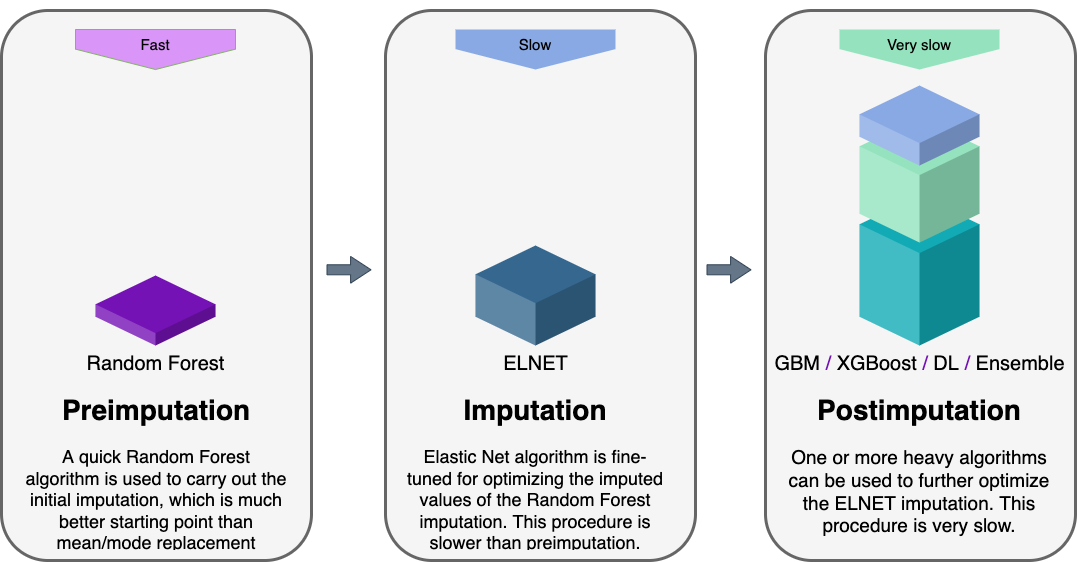
\includegraphics[scale=0.35]{figures/procedure3.png}

\subsection{Supported algorithms}

\begin{itemize}
    
    \item \textbf{\color{violet}RF} (Random Forest and Extreme Randomized Trees). This algorithm is only used in \textit{preimputation}, but it can also be used as the main imputation algorithm or \textit{postimputation} (see below for definitions)
    
    \item \textbf{\color{blue}ELNET} (Elastic Net). This is the main default imputation algorithm
    
    \item \textbf{\color{teal}GBM} (Gradient Boosting Machine).  
    \item \textbf{\color{teal}XGB} (Extreme Gradient Boosting, available in Mac OS and Linux).
    \item \textbf{\color{teal}DL} (Deep Learning).
    \item \textbf{\color{teal}Ensemble} (Stacked Ensemble, only works if other algorithms are also present).
\end{itemize}




\section{Fast optimization with \texttt{ELNET}}

As noted earlier, \texttt{mlim} carries out optimization process on preimputed data. The fastest algorithm for optimizing imputed missing data is \texttt{ELNET}, which is also more fair towards imbalanced data and categories with lower prevalence. As shown in the figures below, \texttt{ELNET} optimization already outperforms all other statistical and machine learning single or multiple imputation algorithms available in \textbf{R}. 

\hspace{-30pt}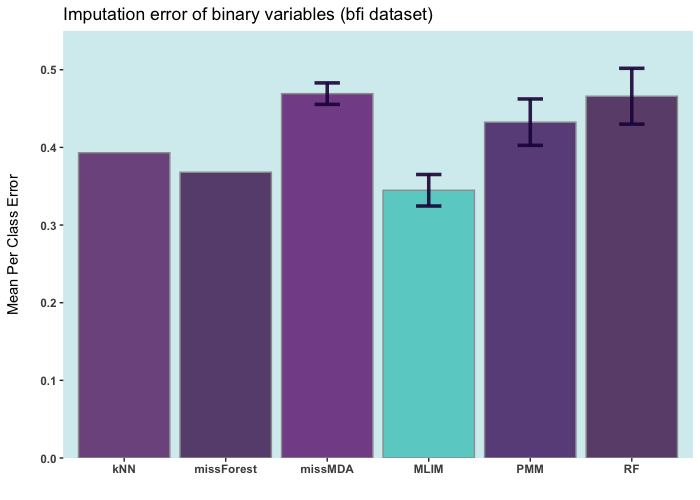
\includegraphics[scale=.3]{figures/bfi_binary_p15.png}
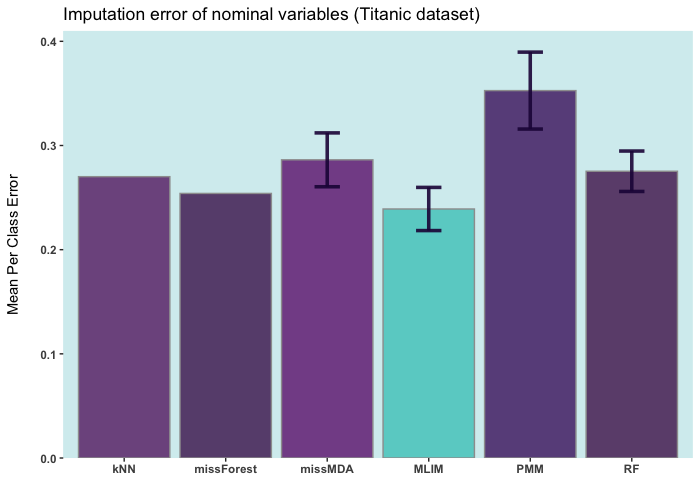
\includegraphics[scale=.3]{figures/titanic_mpce_p15.png}

\hspace{-30pt}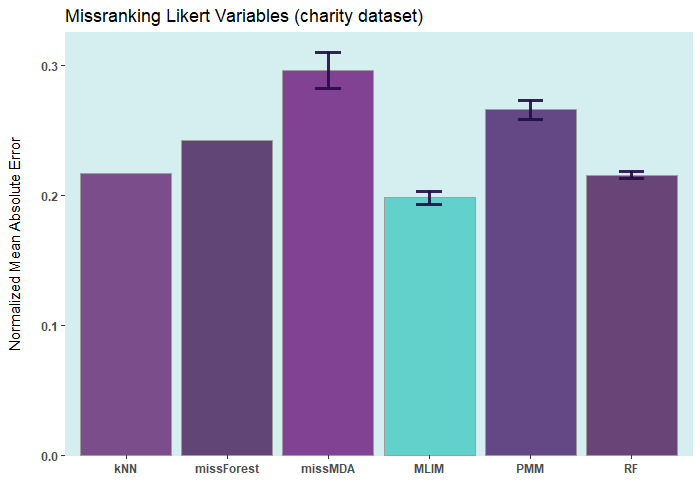
\includegraphics[scale=.4]{figures/charity.png}
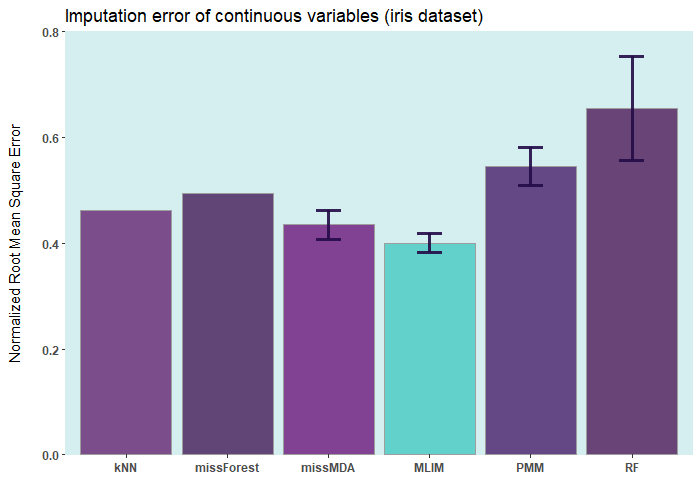
\includegraphics[scale=.4]{figures/iris_continuous_p15.png}

The analysis above uses four different datasets and adds artificial missingness at the rate of 15\% to all variables. Then several famous \textbf{R} algorithms are used to carry out either single or multiple imputation and the results are compared with \texttt{mlim} multiple imputation. There are many imputation algorithms that do not support multiple imputation. In fact, there are many situations where multiple imputation is not feasible or even needed. But as evident in the figures, in all four examples, \texttt{mlim} outperforms all other algorithms for binary, multinomia, ordinal (Likert), and continuous variables.  

\begin{quote}
    \texttt{ELNET} outperforms other R packages and provides fairer imputations  and thus, can result it more reliable single or multiple imputation with less biased estimates, particularly for imbalanced categorical variables. Next, you will see that the performance of \texttt{ELNET} can be further improved with more computationally intensive algorithms. 
\end{quote}

\section{Postimputation with heavier algorithms}

The reason \texttt{mlim} uses \texttt{ELNET} algorithm by default to optimize the imputed observations is that it is easy to fine-tune \texttt{ELNET}, without requiring a huge amount of computing resources or runtime. Moreover, \texttt{ELNET} is a very stable algorithm and generalizes very well, which is a big advantage. On small datasets, other algorithms might simply overfit and even after hours of training, yield less accurate imputed values than \texttt{ELNET} does. However, when desired or needed, the imputed observations can be further optimized with heavier algorithms such as \texttt{GBM}, \texttt{XGB}, \texttt{DL}, \texttt{RF}, or a combination of these algorithms by adding \texttt{Ensemble} (in general, \texttt{Ensemble} is \textit{highly recommended} for stabilizing the postimputation optimization). 

The reader should be aware that postimputation procedure is extremely computation extensive and might not be suitable for standard laptops. If you decide to use strong optimization, make sure you run your analysis on a powerful computer, with a lot of CPU and RAM. The more RAM, the better! If you have 16 GB of RAM, you can still run postimputation, but keep a close eye on the RAM. However, when the data is large enough and the imputation models are well-tuned, the user will be rewarded with significantly lower imputation error and even fairer imputations, which can be of great incentive in some cases. 

\begin{quotation}
    \textbf{Note:} The fact that \texttt{mlim} can do Deep Learning imputation might seem intriguing, i.e., you might think that Deep Learning multiple imputation is more likely to result in a much more accurate single or multiple imputation. Here is a piece of advice: do not underestimate \texttt{ELNET} for its simplicity and speed. Very often, it outperforms other algorithms, while it can be fine-tuned at much faster speed. Comparing the errors of training, other algorithms outperform \texttt{ELNET}, but is there any guarantee that such a reduction of error will be generalizable to the unseen data or the missing values? Answering this question is not that easy. Overfitting can still happen, eventhough \texttt{mlim} performs 10-fold cross validation. Therefore, missing data imputation with heavy machine learning algorithms is a feature intended for advanced users. For general purpose, just use \texttt{ELNET}, which is the default algorithm and you are much more likely to get high efficiency, high accuracy, and even fairer imputed values.  
\end{quotation}

\section{Single imputation}

Traditionally, multiple imputation have been the golden standards if treating missing data because they allow to estimate the uncertainty in guessing the missing observations and that uncertainty is desired. However, multiple imputation is not the only way of making such assessment about the imputed values. Random Forest machine learning algorithm can provide Out Of Bag (OOB) error estimate, which also estimate the prediction error. 

Although \texttt{mlim} can carry out multiple imputation, it can also be used to carry out a single imputation. Yet, \texttt{mlim} can provide estimates of imputation accuracy via Cross Validation metrics. The \texttt{mlim.summarize} function can print the accuracy of the imputation for each imputed variable:


\input{multiple_imputation}

\section{Syntax}

\texttt{mlim} is designed to be suitable for large datasets, despite its computational demands. However, for large datasets, you should be familiar with the syntax of the package as well as the machine you run your analysis on. There are settings for specifying number of CPU cores and RAM. The best place for reading the syntax is the \doclink{https://cran.r-project.org/web/packages/mlim/mlim.pdf}{package Vignette on CRAN}. I avoid reexplaining the syntax of the package because maintaining this document becomes  difficult. Instead, I will focus on the practical aspects of using \texttt{mlim} and thus, for the rest of this document, I will assume that you are familiar with the package syntax. 

\section{Guest authors}

\texttt{mlim} is a free and open-source software, so is its handbook. If you would like to contribute to improving this handbook, even if it's a spelling or grammar check,  \doclink{https://github.com/haghish/mlim_handbook}{fork the repository from GitHub} and help improving it... 


%Code can be printed using the minted or listings packages, or several other tools.
Listing~\ref{listing:octave} shows an example of typesetting code from an external file.

\begin{listing}
\inputminted{octave}{code/BitXorMatrix.m}
\caption{Example from external file}
\label{listing:octave}
\end{listing}

Alternatively, code can be written directly in your .tex files, as in Listing~\ref{listing:py}.
It's also possible to typeset syntax-highlighted code inline with a number of code listing packages.
Check the documentation for the package you're using for more details.
For example, section~3.3 of the \doclink{http://texdoc.net/pkg/minted}{Minted package documentation} gives some examples and guidelines, as does our help article on \doclink{https://www.overleaf.com/learn/latex/Code_Highlighting_with_minted}{code highlighting with minted}. Forums such as \doclink{https://tex.stackexchange.com/}{TeX StackExchange} and \doclink{https://latex.org/forum/}{LaTeX Community} are also a great source of tips.

\begin{listing}
\begin{minted}{python}
print("Hello World")
\end{minted}
\caption{Example Python code}
\label{listing:py}
\end{listing}

%\section{Some further examples to get started}

%\subsection{How to create Sections and Subsections}

Simply use the section and subsection commands, as in this example document. With Overleaf, all the formatting and numbering is handled automatically according to the template you've chosen. If you're using Rich Text mode, you can also create new section and subsections via the buttons in the editor toolbar.

\subsection{How to include Figures}

First you have to upload the image file from your computer using the upload link in the file-tree menu. Then use the includegraphics command to include it in your document. Use the figure environment and the caption command to add a number and a caption to your figure. See the code for Figure \ref{fig:frog} in this section for an example.

Note that your figure will automatically be placed in the most appropriate place for it, given the surrounding text and taking into account other figures or tables that may be close by. You can find out more about adding images to your documents in this help article on \href{https://www.overleaf.com/learn/how-to/Including_images_on_Overleaf}{including images on Overleaf}.

\begin{figure}
\centering
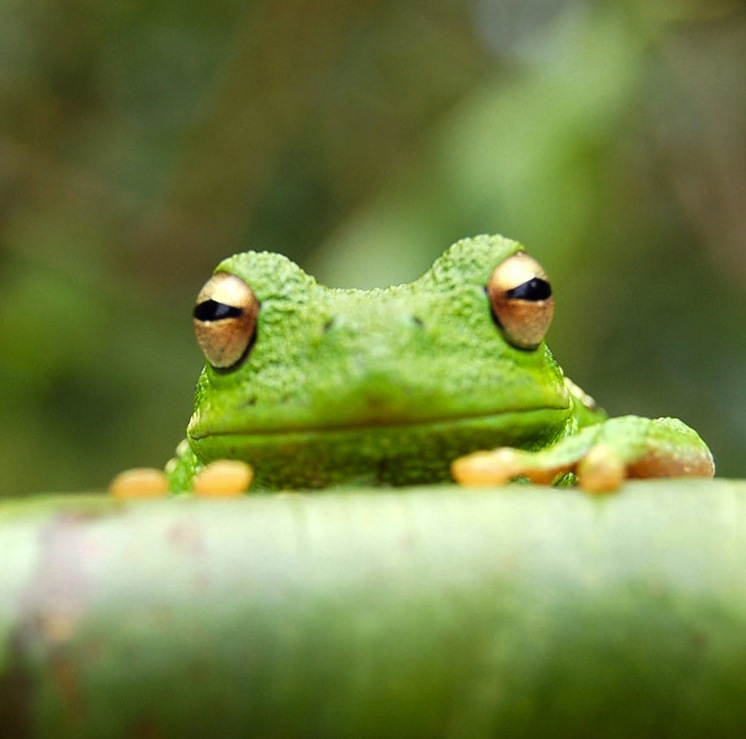
\includegraphics[width=0.3\textwidth]{frog.jpg}
\caption{\label{fig:frog}This frog was uploaded via the file-tree menu.}
\end{figure}

\subsection{How to add Tables}

Use the table and tabular environments for basic tables --- see Table~\ref{tab:widgets}, for example. For more information, please see this help article on \href{https://www.overleaf.com/learn/latex/tables}{tables}. 

\begin{table}
\centering
\begin{tabular}{l|r}
Item & Quantity \\\hline
Widgets & 42 \\
Gadgets & 13
\end{tabular}
\caption{\label{tab:widgets}An example table.}
\end{table}

\subsection{How to add Comments and Track Changes}

Comments can be added to your project by highlighting some text and clicking ``Add comment'' in the top right of the editor pane. To view existing comments, click on the Review menu in the toolbar above. To reply to a comment, click on the Reply button in the lower right corner of the comment. You can close the Review pane by clicking its name on the toolbar when you're done reviewing for the time being.

Track changes are available on all our \doclink{https://www.overleaf.com/user/subscription/plans}{premium plans}, and can be toggled on or off using the option at the top of the Review pane. Track changes allow you to keep track of every change made to the document, along with the person making the change. 

\subsection{How to add Lists}

You can make lists with automatic numbering \dots

\begin{enumerate}
\item Like this,
\item and like this.
\end{enumerate}
\dots or bullet points \dots
\begin{itemize}
\item Like this,
\item and like this.
\end{itemize}

\subsection{How to write Mathematics}

\LaTeX{} is great at typesetting mathematics. Let $X_1, X_2, \ldots, X_n$ be a sequence of independent and identically distributed random variables with $\text{E}[X_i] = \mu$ and $\text{Var}[X_i] = \sigma^2 < \infty$, and let
\[S_n = \frac{X_1 + X_2 + \cdots + X_n}{n}
      = \frac{1}{n}\sum_{i}^{n} X_i\]
denote their mean. Then as $n$ approaches infinity, the random variables $\sqrt{n}(S_n - \mu)$ converge in distribution to a normal $\mathcal{N}(0, \sigma^2)$.

\subsection{How to customize the template}

You may wish to customize the template for your own style, or to meet the specific needs of your documentation. If you're already familiar with LaTeX,  you can go ahead and add the packages you're familiar with to the document preamble. If you run into any problems and can't find the answers in the package documentation or in the Overleaf \doclink{https://www.overleaf.com/learn}{help library}, the forums such as \doclink{https://tex.stackexchange.com/}{TeX StackExchange} and \doclink{https://latex.org/forum/}{LaTeX Community} are a great source of answers.

Some details on how to customize a .cls file (which sets the layout and overall format of the various elements of the template) can be found at \doclink{https://www.overleaf.com/learn/latex/Writing_your_own_class}{Writing your own class}, and \doclink{http://texdoc.net/pkg/clsguide}{\LaTeX2e\ for class and package writers}. 



\end{document}
